\section{Mote Harness}
\label{sec:mote_harness}

In order to guarantee that both sender and receiver will not move during experiments a mote harness was developed and laser cut out of acrylic.
The mote snaps into the harness so that the axis of rotation goes through the middle of the PCB antenna which then allows rotation in \SI{5}{\degree} steps as shown in Figure~\ref{fig:mote_harness}.
Furthermore, the distance between two harnesses can be adjusted in \SI{5}{\milli\metre} steps using laser-cut wooden distance bars.

In our experiments this greatly improved the handling of the motes. Where before we used to tape the mote down into position, which was an inaccurate matter at best, we now have a simple and elegant solution.
However, we ended up not actually using the distance bars in most of our experiments, as it was simpler to use antenna orientation to control link quality than distance.
Therefore, in Figure~\ref{fig:box_hardware_picture} the mote harness is fixed onto the baseplate.

\begin{figure}[t]
	\subfigure[Harness with mote on a distance bar.] {
		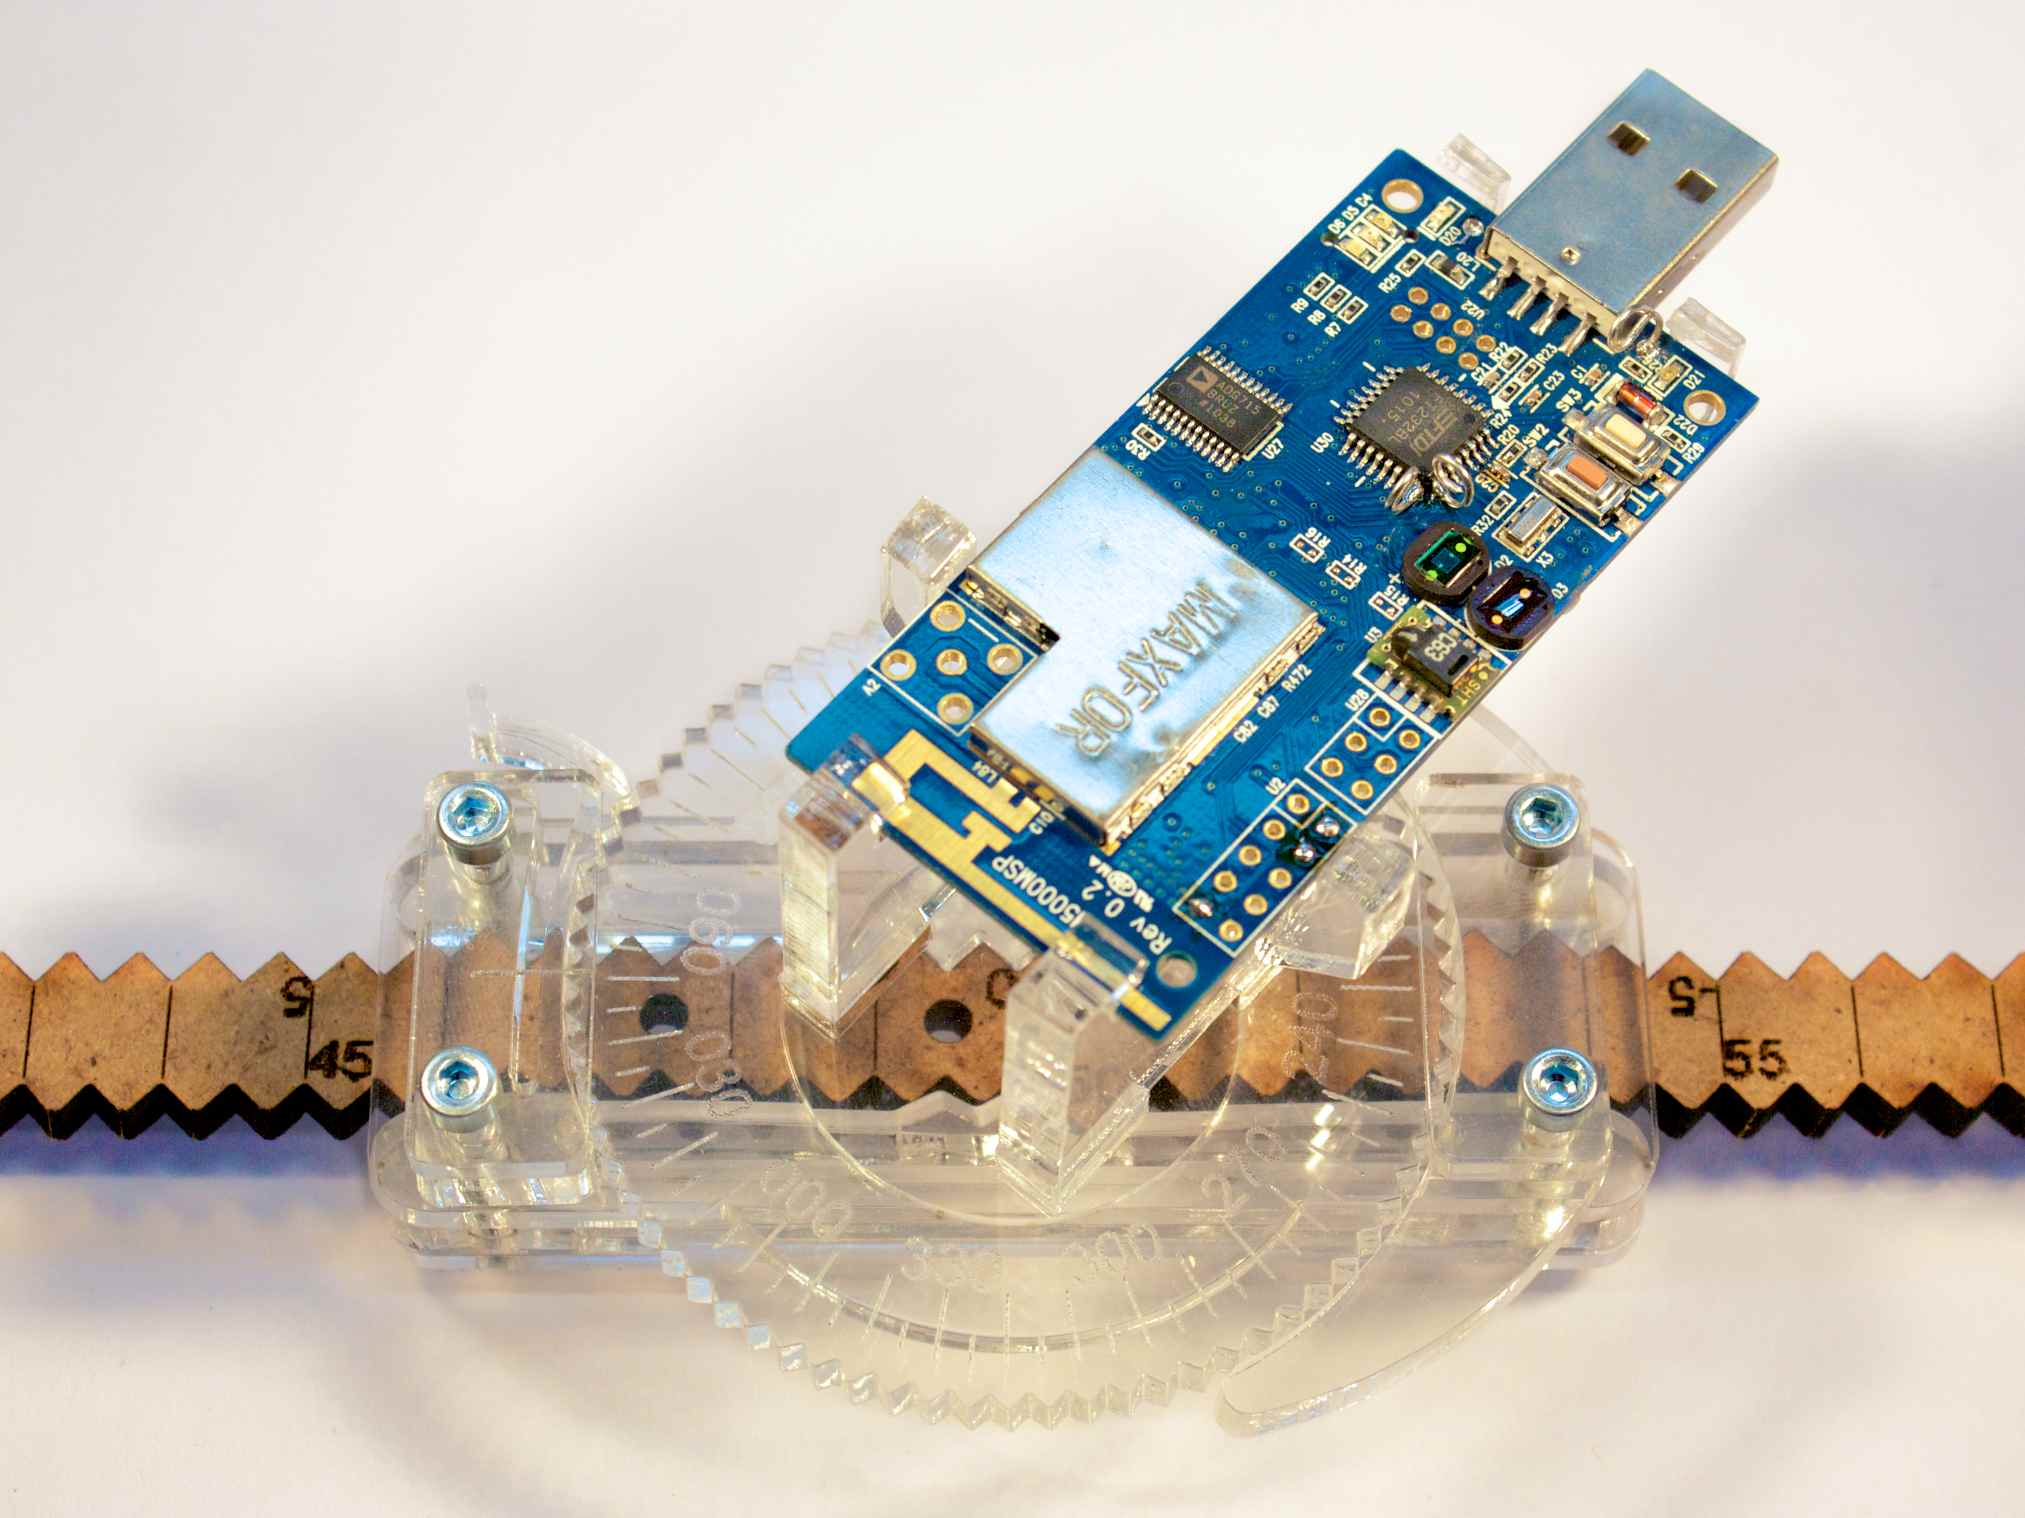
\includegraphics[width=0.5\columnwidth]{figures/harness_picture}
		\label{fig:harness_picture}
	}
	\subfigure[Vector drawing of the rotation disc.] {
		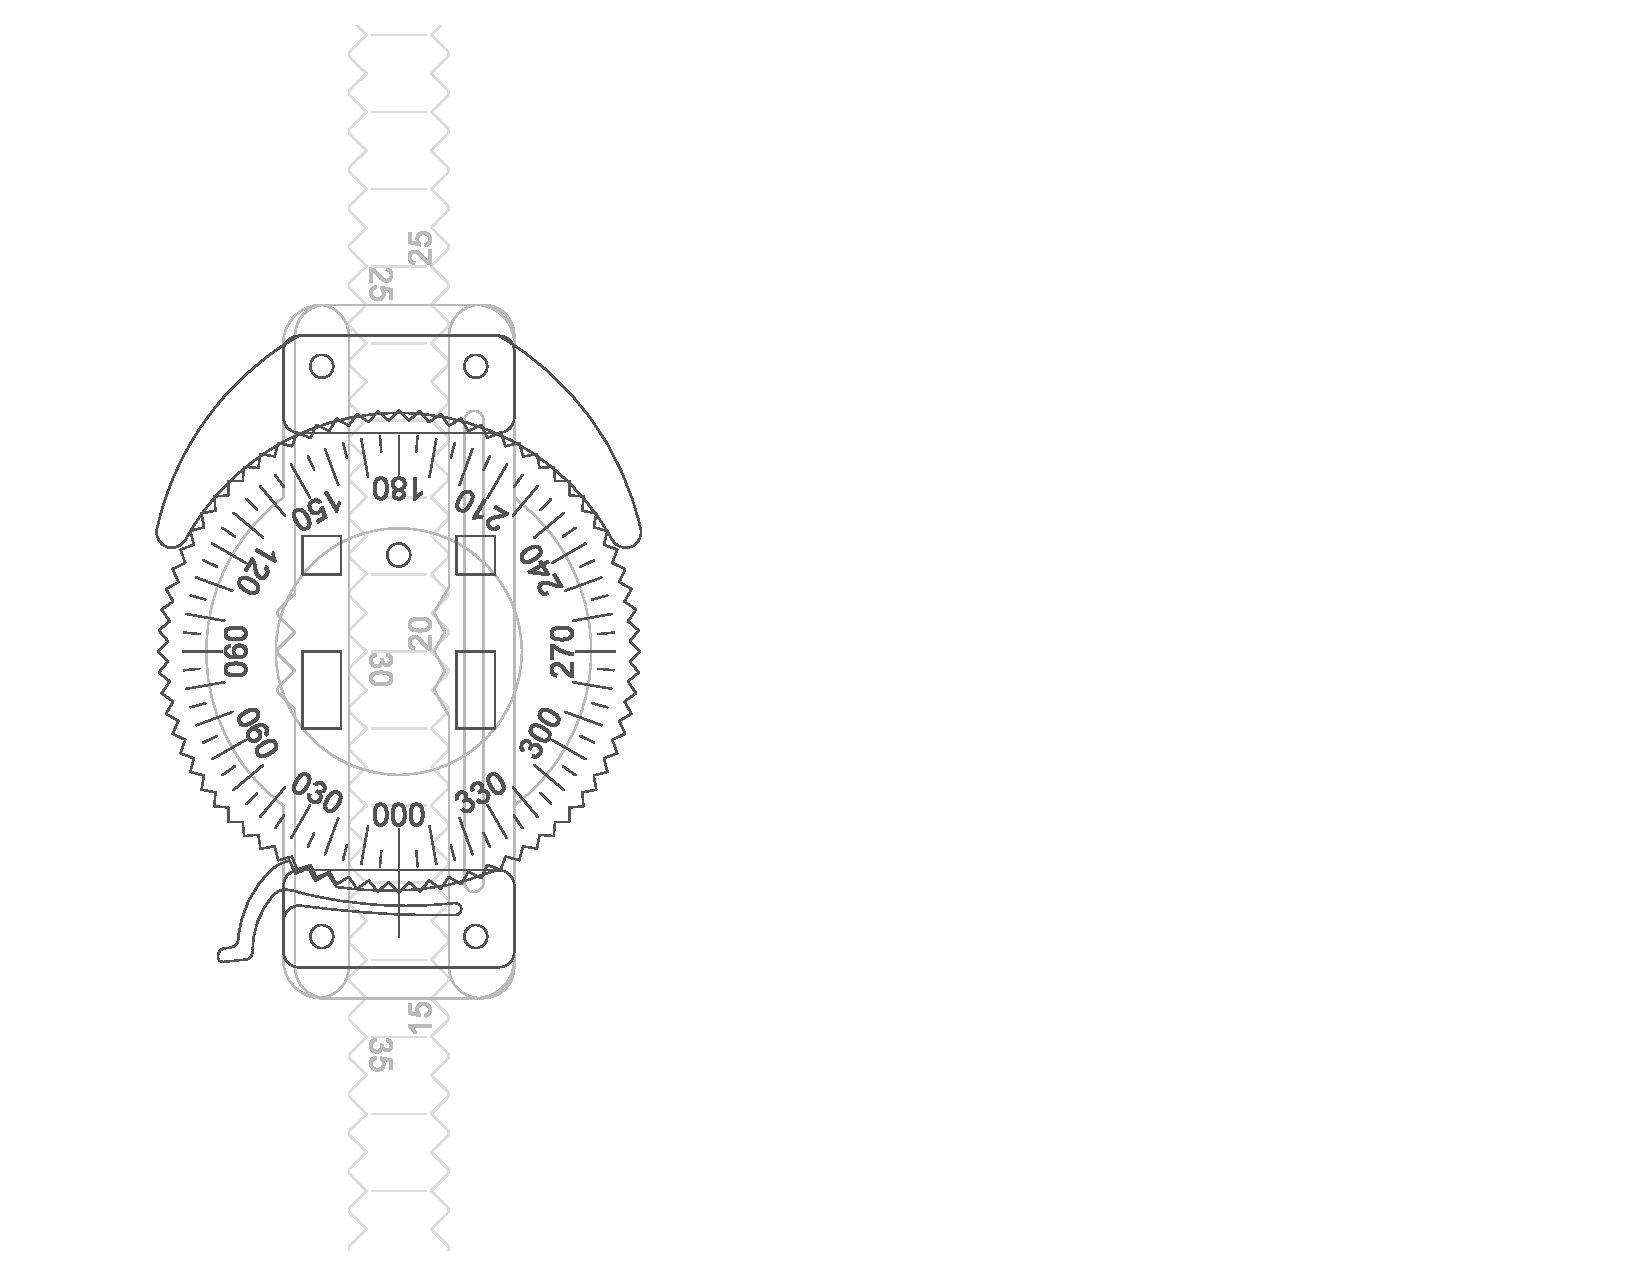
\includegraphics[trim = 20mm 40mm 140mm 45mm, clip, width=0.5\columnwidth, angle=90, scale=0.75]{figures/harness_vector_bar_2}
		\label{fig:harness_vector}
	}
	\caption{The mote harness allows precise positioning of motes.}
	\label{fig:mote_harness}
\end{figure}

% \newpage
